\chapter{基于传统特征与深度特征融合的无线调制方式识别技术研究}
\section{引言}
在机器学习领域,使用特征融合方法解决分类或者回归等问题。
特征融合主要是基于信息融合思想,通过融合不同特征对于问题的不同表征形式,
从不同层次、不同特征空间、不同时间尺度、差异性全局特征和局部特征等不同层面,对特征进行重新组合,
来提高模型的精度和鲁棒性。\par

在上一章中,我们分别展示了CAE以及CNN对调制信号所提取特征的类可分性,即我们可以利用CNN提取数据样本的类别特征。
在本章中,我们将CAE-CNN算法提取的卷积特征与传统特征进行融合,研究深度特征与传统特征结合对分类准确率的影响;
同时,我们也对不同的特征融合框架进行探索,研究不同的融合方式对于特征融合效果的影响。\par

\section{传统特征}

统计模式识别分类方法的研究重点是特征提取方法和分类准则的选择与训练。
不同调制方式我们所提取的特征主要包括:时域特征、频域特征、高阶统计量、循环平稳特性等。
本章针对这几类特征集中的部分特征,利用原始数据进行提取,作为特征融合的传统特征集。\par

\subsection{基本时频特征}

我们假设原始信号$x(t)$解析表示为:
\begin{equation}
s(t)=x(t)+i*y(t)
\end{equation}
其中,$y(t)$为实信号的希尔伯特(Hilberrt)变换。\par

通信信号的瞬时幅度、瞬时频率和瞬时相位等时域特征包含了丰富的调制信息,合理选择和构造它们的各阶统计量是获得调制识别特征的有效途径。\par

\textbf{1)零中心归一化瞬时幅度谱密度的最大值}
\begin{equation}
\gamma_{max}=max|DFT(A_{cn}(t))|^{2}/N_s
\end{equation}
其中,$N_s$为取样点数,$A_{cn}(t)=A(t)/m_a-1$为零中心归一化瞬时幅度,
$m_a=\frac{1}{N_s}\sum_{i=-1}^{N_s}A(t)$为瞬时幅度$A(t)$的平均值,
用平均值对瞬时幅度进行归一化的目的是消除信道影响。$\gamma_{max}$表征了信号瞬时幅度的变化情况,反映调制信号包络的变化特性,可以通过一定的判别门限,区分恒定包络和非恒定包络的信号。


\textbf{2)零中心归一化非弱信号瞬时幅度标准差$\delta_{da}$}
\begin{equation}
delta_{da}=\sqrt{\frac{1}{C}\left[\sum_{A_n(i)>a_t} A_cn^2(i)\right]
	- \left|\frac{1}{C} \sum_{A_n(t)>a_t} A_cn(i)\right|}
\end{equation}
其中,$C$是全部N个采样数据中属于非弱信号值的个数,非弱信号是指幅度大于幅度判决门限电平$a_t$的信号。
$\delta_{da}$表征一个符号区间内信号的幅度变化信息,可以用来区分一个符号区间内归一化中心瞬时幅度的调制方式和归一化中心瞬时幅度不为零的调制方式。


\textbf{3)零中心归一化瞬时幅度绝对值的标准差$\delta_{aa}$}
\begin{equation}
delta_{aa} = \sqrt{\frac{1}{N}\left[\sum_{i=1}^{N} A_{cn}^2(i)\right]
	- \left[\frac{1}{N} \sum_{i=1}^{N} \left|A_{cn}(i)\right|^2\right]}
\end{equation}
$\delta_{aa}$表征了信号的绝对幅度信息,可区分不具备归一化的绝对幅度信息的调制方式,
以及具备归一化的绝对幅度信息的调制方式。


\textbf{4)零中心归一化瞬时幅度的四阶紧致性$\mu_{42}^{a}$}
\begin{equation}
\mu_{42}^{a} = E\left[A_{cn}^{4} (t) \right] / E\left[A_{cn}^{2} (t) \right]
\end{equation}
$\mu_{42}^{a}$是用来度量“瞬时幅度分布的密集性”的特征值,
可以用来区分瞬时幅度高密集分布信号和瞬时幅度分布比较分散的信号。


\textbf{5)零中心归一化瞬时频率均值的平方与方差之$R_f$}\par
\begin{equation}
R_f = u_f^2 / d_f
\end{equation}
式中,$u_f$和$d_f$分别代表信号零中心归一化瞬时频率均值和方差。
此参数可用来判断信号是否含有频率信息。


\textbf{6)零中心非弱信号段归一化瞬时频率绝对值的标准差$\delta_{af}$}

\begin{equation}
\delta_{af} = \sqrt{\frac{1}{c}\left[\sum_{a(i)>a_i} f_N^2(i)\right]
	- \frac{1}{c}\left[\sum_{a(i)>a_i} \left|f_N(i)\right|^2\right]}
\end{equation}
$\delta_{af}$表征信号的绝对频率信息,可用来区分归一化中心瞬时频率绝对值为常数的调制方式和
具有绝对、直接频率信息的调制方式。

\subsection{高阶累积量}

由于码元序列的高阶统计量能够反映星座图的分布特征,适合于区分幅度相位调制方式,并具有抗噪声等优点,
因此基于高阶统计量特征的调制识别算法也是一类有效的分类算法。\par

对于零均值的高斯白噪声信号,三阶及三阶以上的高阶累积量为零。
根据这一特性,求取接收信号$r(t)$的高阶累积量就是求取发送信号$s(t)$的高阶累积量。
从而高阶累积量在对零均值高斯白噪声具有有效的抑制作用以及其它一定程度上的干扰抑制。
对于不同数字调制信号的高阶累积量的值不同,而且不受零均值高斯白噪声的影响,
因此可以有效提取数字调制信号的高阶累积量为特征值,进而区分识别不同信号的调制方式。\par

对于零均值的平稳随机过程$x(t)$,其$k$阶矩定义为:\par
\begin{equation}
M_{kx} = \tau_1, \tau_2, ... \tau_{k-1} = E{x(t), x(t+\tau_1), ..., x(t+\tau_{t+\tau_{k-1}})}
\end{equation}

若考虑延时$\tau_1 = \tau_2 = ... = \tau_{k-1} = 0$,则$x(t)$的$p$阶混合矩:
\begin{equation}
M_{pq} = E\left\lbrace \left[ x(t)\right]^{p-q} 
\left[ x^*(t)\right]^{q}\right\lbrace 
\end{equation}
其中,$x^*(t)$为$x(t)$的共轭,$E{*}$为求期望。\par
根据文献[9]中的高阶矩与高阶累量的定义,我们由零均值的平稳随机过程$x(t)$的各阶累积量的公式。
二阶累积量:
\begin{equation}
\begin{aligned}
C_{20} = Cum(X, X) = M_{20} = E[X(t)X(t)]\\
C_{21} = Cum(X, X^*) = M_{21} = E[X(t)X^*(t)]	
\end{aligned}
\end{equation}

四阶累积量::
\begin{equation}
\begin{aligned}
C_{40}=Cum(X, X, X, X) = M_{40} - 3M_{20}\\
C_{41}=Cum(X, X, X, X^*) = M_{41} - 3M_{20}M_{21}\\
C_{42}=Cum(X, X, X^*, X^*) = M_{42} - M_{20}^2 - M_{21}^2
\end{aligned}
\end{equation}

六阶累积量:
\begin{equation}
\begin{aligned}
C_{60}=Cum(X, X, X, X, X, X) = M_{60} - 15M_{40}M_{20} + 30M_{20}^3\\
C_{63}=Cum(X, X, X, X^*, X^*, X^*) = M_{63} - 9M_{42}M_{21} 
+ 9\left|M_{20}\right|^2M_{21} + 12M_{21}^3
\end{aligned}
\end{equation}

四阶累积量与二阶累积量之比:
\begin{equation}
R_{mn} = |\frac{C_{42}}{C_{21}}|
\end{equation}
 

\subsection{专家循环矩特征}

传统的信号分析模型都是以平稳随机过程为基础的,而通信信号经过调制、周期性采样、编码等具有周期平稳性。
循环统计量可以很好地刻画通信信号的这种周期性。
基于综合循环矩特征[1]目前广泛流行的调制识别和形成分析导出的决策树调制分类到不同的类别。 
一般来说,它们采用方程 \ref{subsec:eq1} 给出的形式。

\begin{equation}
\label{subsec:eq1}
snm = f_{m}(x^{n}(t)...x^{n}(t + \tau))
\end{equation}

通过计算关于瞬时或时间延迟的接收信号$r(t)$的$n$次方的第$m$阶统计量,
我们可以获得一组统计量,该统计量在给定特征的决策过程的情况下将其与其他调制方式唯一地分开。 
对于我们的专家功能集,我们计算32个功能。 这些由0和8个样本的循环时间滞后组成。 
复数接收信号的前2个功率的前2个时刻,每个时滞的幅度,相位和相位的绝对值。\par


\section{特征融合理论}
传统的模式分类方法,主要通过特征提取,利用支持向量机、人工神经网络等算法进行分类器训练。 
但是,传统的模式分类方法通常基于人工设计的特征,经过特征提取算法得到原始数据的某些方向特征,
由于人们对于数据本身认知的片面性,很难利用特征完整的表征数据。
这样,纯粹的基于人工特征提取训练的分类器就无法输出正确的分类。\par

解决此问题的一种思路就是使用特征融合算法,利用多维特征构成的特征空间,来获取数据本身包含的性质,
,弥补某些固有特征对于数据特征反映不完整的缺陷。
特征融合方法从特征层面进行处理,它既可以直接利用已有的算法提取数据特征,
相较于重新设计特征和特征提取的算法,具有较低的成本。
在本节中,我们主要研究基于深度学习的特征融合理论。\par

深度学习理论是在人工神经网络的基础上发展起来的机器学习理论,在多层神经网络中加入了更多隐层单元。
基于深度学习的特征融合算法,主要是对深度神经网络模型引入特征融合的思想,
并在模型中选择特定隐层融合其他特征,利用多源特征来训练网络参数。\par

特征融合理论主要基于两个基本假设:
\begin{quote} 
	1) 多特征融合通常比单特征具备更好的分类性能;\\
	2) 融合的特征之间相关性尽量小。
\end{quote}

前者是进行特征融合的出发点和前提,只有融合后的特征具备这样的特性,我们才具备融合的必要性。
后者是基于流形理论的假设,当特征之间的关联性较高时,融合之后的特征空间在高维流形中趋于扁平化,
可能会产生特征冗余,我们实际上可以用更小的维度来表征原始数据。
因此,我们应该从多角度选择低相关性的特征进行融合,
使数据能够在融合特征形成的高维流形中处于一个有利于我们任务(分类、回归等)的分布。\par

假设原始的数据样本集为$X$,那么对于任意${x \in X}$,
我们假设用于提取特征的隐层单元集合为$H_{hidden}$,其维度为$N$,
$h_i(x)$表示网络中第$i$个单元的输出值,则隐层神经单元构成的深度特征集为$H={h_i(x)|h_i \in H_{hidden}}$。
通过深度网络,我们可以获取原始特征空间到深度特征空间的映射:
\begin{equation}
	h(x) = \bigcup_{0<i<N} w_i * h_{i}(x)
\end{equation}
当数据通过网络映射到深度特征空间的输出值,便是我们在新空间中的特征向量,即数据的深度特征。\par

同时,我们以本章中第2小节的特征提取算法,对数据的传统特征进行提取,每一个特征用$f_{i}(x)$表示,作为不同维度的特征,假设我们的传统特征集为$F$,对于任意样本$x \in X$,我们根据第2小节中的特征提取算法有:
\begin{equation}
	f(x) = \bigcup_{0<i<|Z|}\mu_{i} * f_{i}(x)
\end{equation}

这样,通过融合传统特征$F$与深度特征$H$得到的融合特征集为$Z$:
\begin{equation}
	Z =F \cup H = \{ z | (z \in H) \vee (z \in F) \}
\end{equation}
最终,我们通过不同的融合算法对多源特征进行融合。特征融合的基本框架如图\ref{sec:fig_4_1}所示:

\begin{figure}[!h]
	\centering
	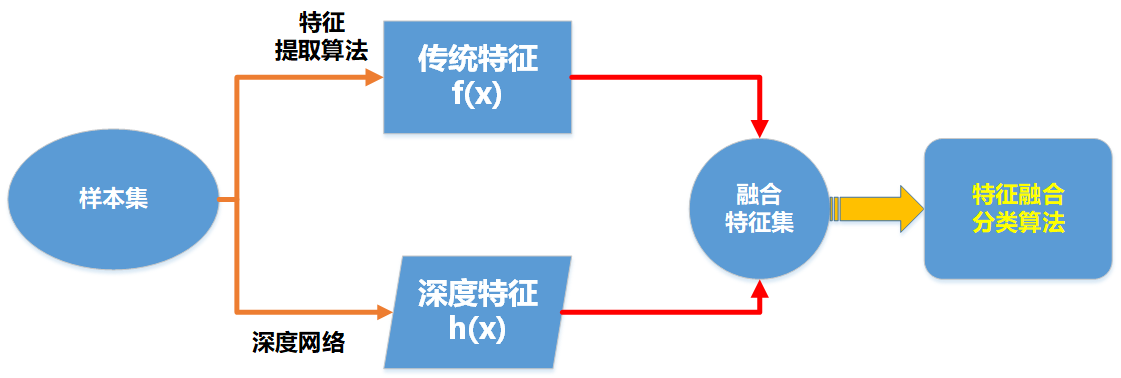
\includegraphics[scale=0.5]{figures/chapter_4/fea_combine.png}
	\caption{特征融合框架图}\label{sec:fig_4_1}
\end{figure}

其中,XX表示我们利用的不同融合算法。在下一节中,我们将对不同融合算法的效果进行研究。


\section{传统特征与深度特征融合框架}

基于统计模式的调制识别方法也称为基于特征的调制识别方法。
这种方法把通信信号的调制
识别视为一个统计模式识别问题,整个调制识别系统由两个子系统组成:
特征提取子系统和模式分类子系统。
特征提取子系统的作用是从原始测数据中提取事先定义好的能表征信号调制类型的特征,
可以看作是从输入信号所在的观测空间到选定的特征空间的一个映射。\par

\subsection{基于Softmax回归(Softmax Regression, SR)的融合框架}
LR是用线性回归模型的预测结果去逼近真实标记的对数几率的一种二分类算法。SVM是一种基于核函数的方法,它通过某些核函数把特征向量映射到高维空间SVM是一种基于核函数的方法,它通过某些核函数把特征向量映射到高维空间,然后建立一个线性判别函数对数据进行分类。由于SVM训练时间较长,而线性核函数的SVM与LR的结果基本一样【吴恩达】,因此,为了兼顾算法的有效性和高效性,我们选择LR框架作为线性特征融合的框架。\par

根据【吴恩达】,我们有样本为正样本的概率:

\begin{equation}
	h_{\theta}(x) = p(y=1|x) = \frac{1}{1 + e^{-(\theta^T x)}}
\end{equation}

我们用$Cost(h_{\theta}(x^{(i)}), y^{(i)}) $表示样本预测错误时的损失,
根据【】,在此我们使用逻辑损失函数:
\begin{equation}
		Cost(h_{\theta}(x^{(i)}), y^{(i)}) = 
			\begin{cases}
				-\log(h_{\theta}(x^{(i)})) & \text{$y = 1$}\\
				-\log(1 - h_{\theta}^{(i)}) & \text{$y = 0$}
			\end{cases}
\end{equation}

最终,我们有LR的损失函数:
\begin{equation}
	\begin{aligned}
		J(\theta) &=- \frac{1}{m} \sum_{i=1}^{m} Cost(h_{\theta}(x_{(i)}), y_{(i)})\\
			&= -\frac{1}{m} \sum_{i=1}^{m} \left[
				y^{(i)} \log(h_{\theta}(x^{(i)})) +
				(1 - y^{(i)})\log(1 - h_{\theta}^{(i)})
			\right]
	\end{aligned}
\end{equation}

由于,我们传统的LR算法针对的是二分类问题,因此,对于调制识别这样的多分类问题,我们需要对算法进行改进。
在此,我们使用的是LR多分类算法中的$1VM$版本【】,即假设我们的调制类别共有$M$类,则我们需要训练$M$个分类器,分别判断样本属于每一个类别的概率值,取概率值最高的那一个类别作为我们的分类结果。\par
最终的基于LR的特征融合框架,如图\ref{sec:fig_4_2}所示:
\begin{figure}[!h]
	\centering
	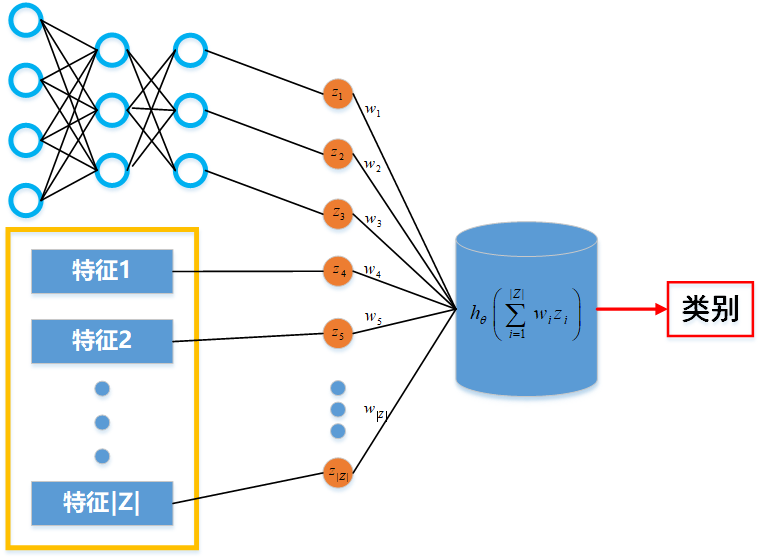
\includegraphics[scale=0.7]{figures/chapter_4/LR_combile}
	\caption{基于LR框架的特征融合框架图}\label{sec:fig_4_2}
\end{figure}


\subsection{基于深度学习的融合框架}
随着深度学习的发展,已经有部分学者对基于深度学习的特征融合方法进行了研究。
Simonyan 等[16]首先提出了一种使用双流架构的深度卷积神经网络模型,可解决视频中的动作识别问题。
Feichtenhofer 等[15]则在这个基础上改进了网络融合方法,提出了空间特征融合方法和时间特征融合算法。\par

“如果我们的深度网络达到一定的条件,可以拟合任意的函数。“,XXX说。
DNN是对输入的数据样本,通过隐层对数据进行非线性变换,利用交叉熵或者均方误差等损失函数对隐层参数进行训练,
来输出我们希望的结果。\par

基于深度学习框架的融合方法,在融合点之前分别进行特征学习。
由本章第3小节定义,通过深度网络学习到的特征集为$H$,通过传统算法提取的特征集为$F$。\par

为降低因为特征尺度关系对后期网络学习造成的影响,我们在特征融合之前在框架中加了一个特征预处理层,
来对特征进行归一化处理。此时,我们获得的归一化特征集变为:
\begin{equation}
	\hat{Z} =\{ f_{norm}(z) | z \in H \cup F \}
\end{equation}

融合层将独立学习的归一化特征进行融合,输入到神经网络中。
XXX等人提出了可以利用卷积层、池化层等对不同的特征进行融合处理。
我们通过对包括LSTM、DNN、CNN等框架进行验证之后,最终使用的是卷积神经网络,
并在其中加入池化层,使用dropout降低模型的过拟合风险。
在之后的深度网络层,由于样本数据有限,我们仅仅用了2层的全连接层,但是从分类结果来看,其效果还是达到预期。\par


整个基于深度学习的特征融合框架如图\ref{sec:fig_4_3}所示:
\begin{figure}[!h]
	\centering
	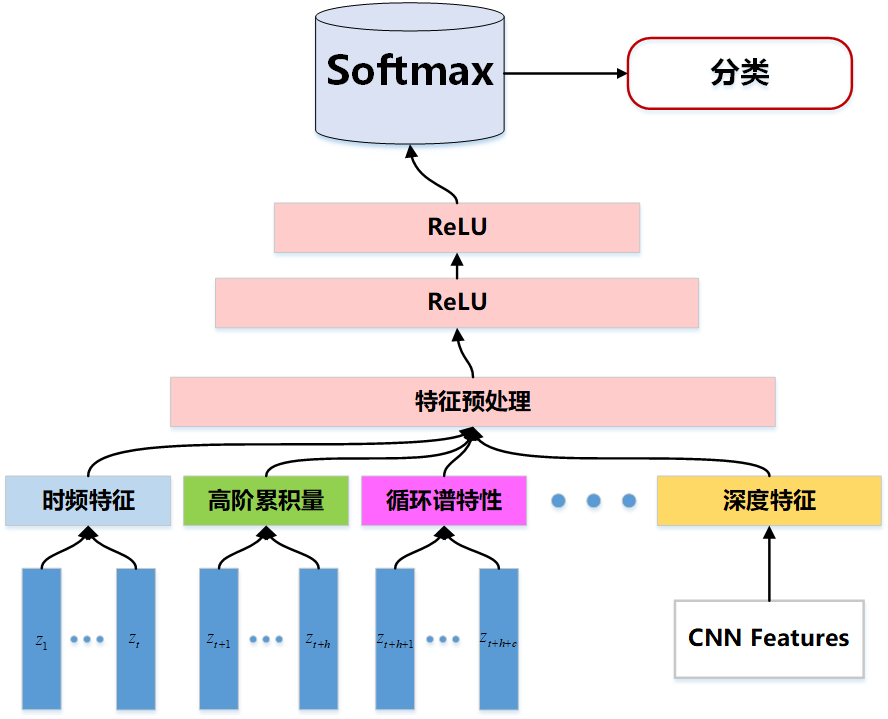
\includegraphics[scale=0.6]{figures/chapter_4/DL_combine}
	\caption{基于DNN框架的特征融合框架图}\label{sec:fig_4_3}
\end{figure}


\subsection{基于随机森林的融合框架}
集成学习通过构建并结合多个基学习器来完成学习任务,按照算法的思想它主要分为两类:Bagging族算法和Boosting族算法。\par

Bagging [Breiman, 1996a] 是一类井行式集成学习的算法,主要基于采样数据集训练基学习器,并对这些基学习器进行组合(比如分类问题投票法、回归问题平均法)作为最终结果。Bagging主要是通过多个基学习器的集成来降低模型的方差。

Boosting算法的思想是先训练简单的基学习器,再根据基学习器的表现对训练样本分布进行调整,
使得先前基学习器做错的训练样本在后续受到更多关注,然后基于调整后的样本分布来训练下一个基学习器,
直至基学习器数目达到事先指定的值T , 最终将这$T$个基学习器进行加权结合。Boosting 主要通过过个学习器的加性组合降低偏差。\par

随机森林(Random Forest,RF) [Breiman, 2001a] 是一个基于Bagging思想的,通过随机方式建立的,包含多棵决策树的集成分类器。
它通过自助法(bootstrap)重采样技术,从原始训练样本集N中有放回地重复随机抽取k个样本生成新的训练样本集合,然后根据自助样本集生成k个分类树组成随机森林,新数据的分类结果按分类树投票多少形成的分数而定。对于我们的调制分类任务而言,随机森林简单、容易实现、计算开销小,正符合我们对集成树融合效果的验证性要求。\par


对于调制分类问题,我们将CART树【】作为基分类器,并引入样本采样和特征采样,增加样本扰动和特征扰动对集成学习算法的影响。
基分类器的集成方法主要有平均法、投票法、stagging学习法等方法,
平均法主要是针对回归问题,而stagging的方法是利用基分类器的输出作为新的样本学习一个新的分类器,会增加模型的复杂度。
因此,在调制分类问题中,我们使用投票法来作为基分类器的结合方法。\par

假设我们总共学习$K$个基学习器,则每个并行训练得到的基学习器为$T_{i}$,
那么利用投票法所得的分类结果如方程\ref{sec:eqt_4_23}所示:
\begin{equation}
	C(x) = \mathop{\arg\max}_{c} \sum_{i=1}^{K} I(T_i(x), c)
\end{equation}

其中,$I(T_i(x), c) \in \{0, 1\}\}$,若基分类树$T_{i}$将样本$x$预测为类别$c$,则$I(T_i(x), c)=1$,否则$I(T_i(x), c)=0$。\par
RF不仅通过样本扰动(通过对原始训练集进行采样)实现随机性,
而且通过对属性进行随机采样来增加特征的扰动,通过多棵数进行投票来预测分类结果。
这就使得最终的集成分类器的泛化性能,可通过个体学习器之间差异度的增加而进一步提升。\par
图\ref{sec:fig_4_5}展示了我们基于随机森林算法的特征融合框架图:
\begin{figure}[!h]
	\centering
	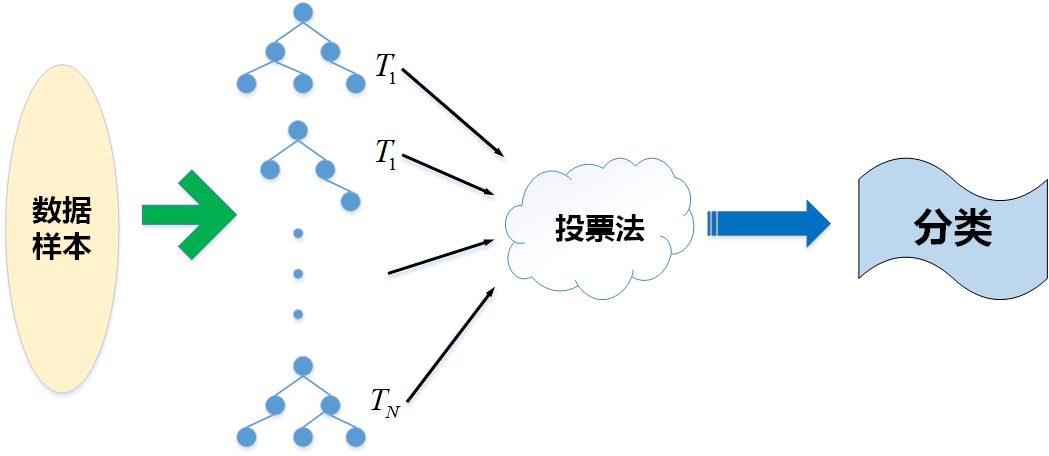
\includegraphics[scale=0.5]{figures/chapter_4/Tree_combine}
	\caption{基于随机森林框架的特征融合框架图}\label{sec:fig_4_4}
\end{figure}



。随机森林(RandomForest,RF)基于划分与模型融合的方法。降低了泛化误差。

\section{结果及分析}

\subsection{分类性能比较}
我们利用11类数据对三种框架的模型进行训练,对于不同框架模型的超参数如表【】所示:
、、、、、、、、、、、、
、、、、、、、、、、、
最后的分类结果如图【】所示:

\begin{figure}[!h]
	\centering
	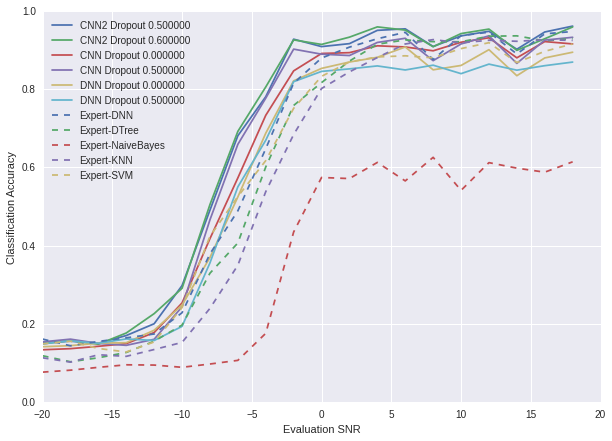
\includegraphics[scale=0.3]{figures/chapter_3/result}
	\caption{不同融合框架下的分类性能对比}\label{fig_2_2}
\end{figure}

通过上图,我们可以发现在高信噪比条件下,三种框架的差别并不太大,但是利用深度CNN的融合框架更好一些,可能是因为这种情况的拟合能力更强一些,由于训练数据本身具有较小的噪声,所以对于强拟合能力的模型而言,泛化误差影响相对较小;
在0dB时候,三种框架的性能有:A》B》C;
在信噪比低于》》》时,XX的性能更好一些,因为RF是通过随机的样本采样和特征采样来降低泛化误差,对噪声数据相对不敏感一些。

\subsection{混淆矩阵}

\subsubsection{RF混淆矩阵}

\subsubsection{DNN混淆矩阵}

\subsubsection{SR混淆矩阵}

仔细检查这些结果,我们可以看到BPSK不幸与QPSK和8PSK调制(它是其中的一个子集)相当混杂。
然而,QAM16是一个以前看不见的类,这些特征在QAM64附近紧密聚集在一个相当明确的可分离的嵌入空间区域。
这些结果虽然非常初步和定性,但确实支持这一事实,即自举特征映射具有显着的泛化能力,
能够识别,聚类和辨别新的未知的或以前看不见的调制类型,但是并不保证在所有情况下都具有清晰的可分离性。
我们希望随着类别和特征数量的增加,这种泛化将会得到改善。
推进这一研究领域的挑战之一将是确定和量化特征总结能力的衡量标准,并着力于改进这一指标。\par

\section{本章小结}


在这项工作中,我们已经证明,使用原始采样无线电时间序列数据上的卷积神经网络学习的低级别时间序列特征可以用于有效地聚类许多无线电信号调制类型,而没有明确标记的训练数据。我们已经表明,通过利用从差异特征映射和压缩重构空间学习的压缩表示,我们可以开始组织和构造复杂的无线电信号数据集与未标记或标记不佳的起点。这是一个强有力的结果,因为它展示了一个潜在的前进方向,可以学习区分,推理,回忆和描述新的和未知的无线电信号,而无需手动指导或专家指导。这是一个关键的要求,因为我们试图建立随着时间的推移而从经验中扩展能力的系统。将压缩的特征空间基础推广到新的信号类型仍然是这个领域的一个关键挑战,但是我们在这项工作中已经表明,在某些情况下这种特征泛化确实发生。展望未来,量化和优化这种效应的尝试将是重要的。\par

特征融合方法是模式识别领域的一种重要方法. 计算机视觉领域的图像识别问题作为一种特殊的模式分类
问题,仍然存在很多挑战. 特征融合方法能够综合利用多种图像特征,实现多特征的优势互补,获得更加鲁棒和准
确的识别结果. 笔者基于信息融合理论分析了特征融合方法的原理,介绍了特征融合方法的研究现状,讨论了特征
融合与 3 类主流基础理论相结合的方法,其中基于贝叶斯理论的特征融合算法可以实现多特征的融合决策,基于
稀疏表示理论的特征融合算法能够得到多特征的联合稀疏表示,基于深度学习理论的特征融合算法能够强化深度
神经网络模型的特征学习过程.\par
